\chapter{Experiments}
The proposed algorithm (MRSM) and the benchmark algorithms (MRSIS \cite{li2024mrsis}, CapAM \cite{paull2022learning}, PD-FAC \cite{sheng2022pd}, and the other 2 methods) are evaluated based on the expected number of detected objects (ENDO) and the expected time to detection (ETTD).
The ETTD is defined as follows:
\begin{equation*}
  E[TTD] = \frac{1}{TO}\sum_{t=1}^{T}\sum_{o=1}^{O}\tau^t_o,
\end{equation*}
where $T$, $O$, and $\tau^t_o$ represent the number of trials, number of objects in trial $t$, and detection time of object $o$ in trial $t$, respectively.
Besides, if the drones fail to detect objects, the search time is set to the maximal time constraint.

The search process is as follows: MRSM generates a set of trajectories composed of $K_i$ edges before the $i^{th}$ drone takes off. As the drone reaches the subgoal, it hovers and detects targets within 3 seconds. The drone continues to traverse the edge and visits the next subgoal. The process continues until all targets in the environment have been identified or all drones have traversed their designated edges.
When the search task is terminated, drones land on the ground.

\begin{figure}[htbp]
\centerline{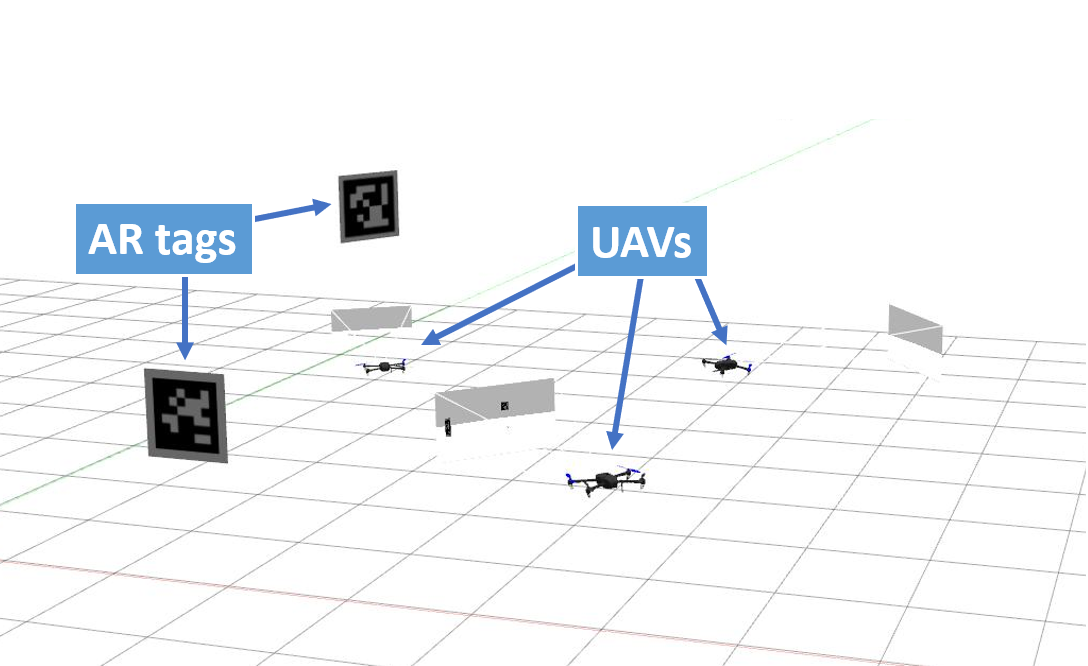
\includegraphics[width=0.65\textwidth]{gazebo-env-1.png}}
\caption{
Gazebo simulation with 3 UAVs and 2 objects (AR Tags) in a 3D Environment.
The UAV can project a viewing frustum to observe the search space.
% A tuple $(e,t)$ represents a pair of space size and number of targets (AR Tags) for search.
% For example, $(8,4)$ stands for the size of $8^3$ with {\color{magenta}2} targets within this environment.
% The red cube represents the robot searching for the target.
}
\label{environment}
\end{figure}

\section{Experiment Setup}
Three experiments are conducted: the target search experiment (EX1), the parametric analysis (EX2), and the scalability analysis (EX3).

In the target search experiment (EX1), the performance of the proposed algorithms (MRSM) is assessed through simulation
(see Fig.~\ref{environment}) and a realistic environment (see Fig.~\ref{GEB_fig}).
The assessment includes a comparison with state-of-the-art approaches (e.g., MRSIS \cite{li2024mrsis}, CapAM \cite{paull2022learning} and PD-FAC \cite{sheng2022pd}).
The simulation is carried out with 3 robots (UAVs) on Gazebo (see Fig. \ref{environment}). Various environment sizes $\mathit{\mathbb{E}}=\{8,12\}$ and numbers of targets (AR tags) $\mathit{\mathbb{T}}=\{2,4,6\}$ in the space are evaluated.
Each $(a,b)$ pair generates 100 trials with randomly located targets,
where $a \in \mathit{\mathbb{E}}$ is an $a \times a \times a (m.)$ search space, and $b \in \mathit{\mathbb{T}}$ is the number of targets in $a$.
The robot's goal is to find all targets in scenarios of partial occlusion.

A weighted graph $\mathcal{G}=(\mathcal{V}, \mathcal{E}, c)$ is constructed to represent the environment, where $\mathcal{V}$ is the subgoal set, $\mathcal{E}$ is the edge set, and $c$ is the routing costs with respect to edges.
The subgoals $\mathcal{V}$ are evenly distributed throughout the space and each subgoal is defined as $v\in \{(x,y,z,\theta)|(x,y,z,\theta)\in \mathcal{V}\}$, where $x,y,z\in[1, e]$ and $\theta\in\{0,60,120,\\180,240,300\}$.

In the search process, each robot can take one of the actions from $\mathcal{A}=\{Move(x,y,z,\theta), Detect\}$.
The $Move$ action takes the drone to the coordinate $(x,y,z)$ with the heading $\theta$.
The $Detect$ action performs an object detection.
The time constraint of the search process is 10 minutes.
Once all the targets have been found or the search time exceeds the constraint, the task is terminated.

The coverage function ($f$) is calculated by the ratio of the number of covered voxels to the total number of environmental voxels. The routing cost ($c$) is measured by the Euclidean distance between two subgoals\footnote{For any two connected nodes, $v_1=(x_1,y_1,z_1, \theta_1)$ and $v_2=(x_2,y_2,z_2,\theta_2)$, the routing cost $c(\{(v_1,v_2)\})=\sqrt{(x_1-x_2)^2+(y_1-y_2)^2+(z_1-z_2)^2+(\theta_1-\theta_2)^2}$.}.

There are two real-world experiments with 2 drones.
The first one is in a 13 $\times$ 9 $\times$ 2 $m$ public area on the third floor of the General Education Building at the National Central University (NCU) (see Fig. \ref{GEB_fig}(a)).
The space is divided into voxels whose unit size is $15 \times 15 \times 15$ $cm$.
The goal is to find a sports ball, a chair, and a bottle in the environment, shown in Fig. \ref{GEB_fig}(b).
Three targets are randomly located and can be partially occluded due to the complex environment with obstacles.
The second one is in a 50 $\times$ 50 $\times$ 5 $m$ Hengshan Calligraphy Art Park (see Fig. \ref{Call_fig}(a)).
The space contains plenty of obstacles (trees). The goal is to find three AR tags in the environment, shown in Fig. \ref{Call_fig}(b).

The searchers are the drones developed by Taiwan Drone 100 shown in Fig. \ref{drone}.
The drone is equipped with NVIDIA Jetson Xavier NX and two Intel RealSense cameras.
The Intel RealSense T265 camera is used to localize the drone and the D435i camera is to explore the environment.
The camera and drone parameters are shown in Table \ref{Tab:parameters}.

To detect objects, the YOLOv5 \cite{glenn_jocher_2022_7347926} is adopted and run on NVIDIA Jetson Xavier NX.
The uncertainty of detection is considered due to object occlusion in the environment. To successfully detect the object, the confidence rate of detection must be over a threshold of 0.6.

In the parametric analysis experiment (EX2), the parameters, the weight of the balancing function ($\lambda$), and the robot routing budget ($l_i$) are investigated for MRSIS \cite{li2024mrsis} and MRSM algorithms within an $8\times8\times8 (m.)$ simulated environment.
Three robots (UAVs) are tasked to find various numbers of targets $b \in \{2,4,6\}$ with different balancing weights $\lambda\in\{0\,,0.2,\,0.4,\,0.6,\,0.8,\,1\}$ and robot routing budgets $l_i\in\{20,\, 40,\, 60,\, 80\}$.
When $\lambda=0$, no balanced workloads are considered.
When $\lambda=1$, the workloads assigned to robots are thoroughly optimized.
The experiment setup is the same as the simulation in EX1.
Additionally, a comparative analysis of computational time is conducted for both methods.

In the scalability analysis experiment (EX3), the performance of MRSM and MRSIS\cite{li2024mrsis} is evaluated under a
$20\times20\times20(m^3)$ simulated space involving a considerable number of robots $R=\{5, 10\}$.
Performance is evaluated on different numbers of subgoals $\mathcal{V}=\{700,800,900\}$.
Robots (UAVs) must find 8 targets (AR tags) in the environment.
The balancing weight $\lambda$ and robot routing budget $l_i$ are set to $0.2$ and $300$, respectively.
The camera range is set to 5 meters and the remaining configurations are established in the same manner as the simulation in EX1.

Two baseline methods (CapAM\cite{paull2022learning} and PD-FAC\cite{sheng2022pd}) are implemented for the search scenarios. In CapAM\cite{paull2022learning}, the state space of the MDP contains features such as the elapsed mission time, the robot's current location, and the robot's work capacity. The action space of the MDP is the action set $\mathcal{A}$. The goal of CapAM\cite{paull2022learning} is to visit as many subgoals as possible.
In PD-FAC\cite{sheng2022pd}, the weighted graph $\mathcal{G}$ maintains the same format as detailed in \cite{sheng2022pd}. The search time budget is set to 10 minutes and the search targets are randomly placed on the graph nodes. Once the robot visits the node on the graph, the target is marked as found. The configurations of PD-FAC can be found in \cite{sheng2022pd}.

\renewcommand{\arraystretch}{1.3}
\begin{table}[h]
\caption{Parameters of EX1 and EX2.}
\begin{center}
\begin{tabular}{|c||c|c|c|}
\hline
Parameters & Simulation & Real-world search \\
\hline\hline
Camera range & $2m$ & $3m$  \\
\hline
Horizontal FOV & $45^{\circ}$ & $69^{\circ}$  \\
\hline
Vertical FOV & $45^{\circ}$ & $42^{\circ}$ \\
\hline
Transitional velocity & $1.3$ $m/sec$ & $0.2$ $m/sec$ \\
\hline
Angular velocity & $45$ $deg/sec$ & $120$ $deg/sec$ \\
\hline
\end{tabular}
\label{Tab:parameters}
\end{center}
\end{table}


\begin{figure}
    \centering
    \begin{subfigure}[b]{0.5\textwidth}
        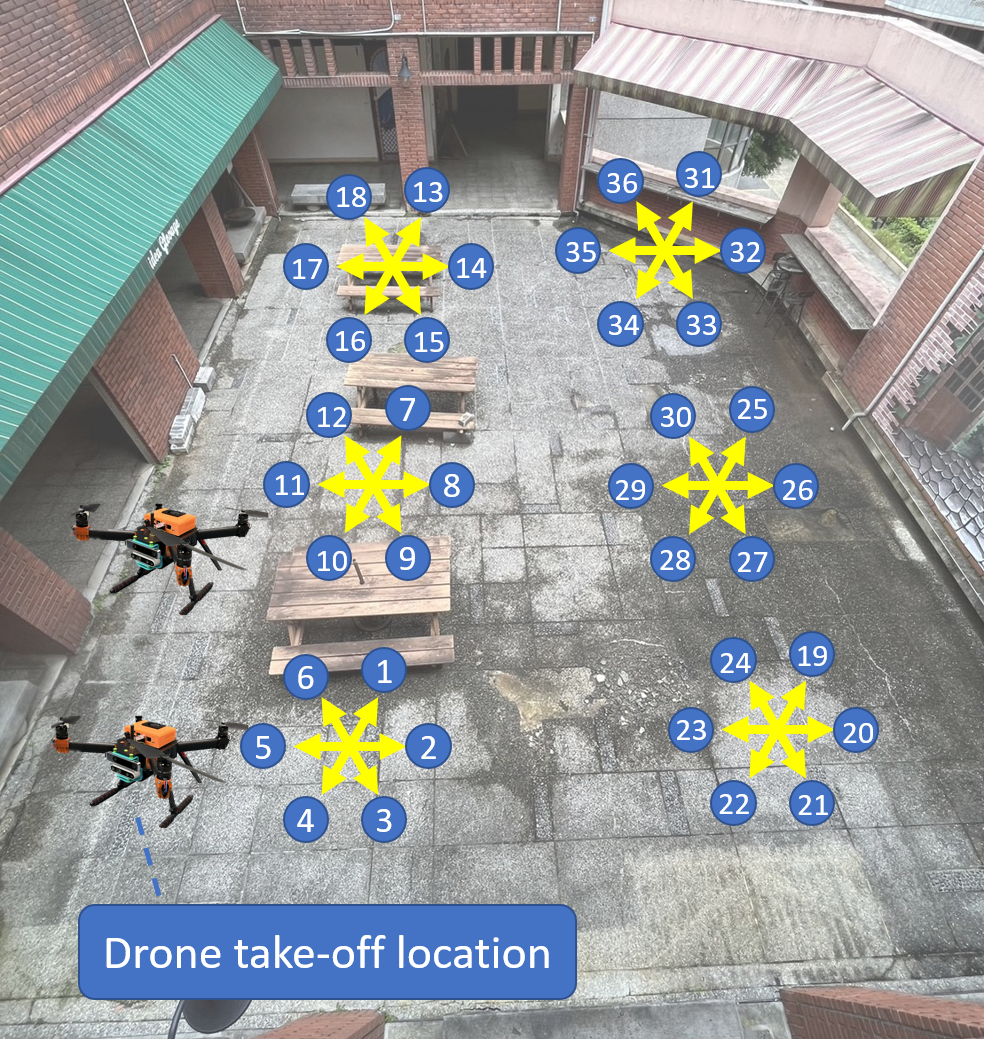
\includegraphics[width=1\textwidth]{GEB.png}
        \caption{} \label{GEB map}
    \end{subfigure}
    \begin{subfigure}[b]{0.5\textwidth}
    \centering
        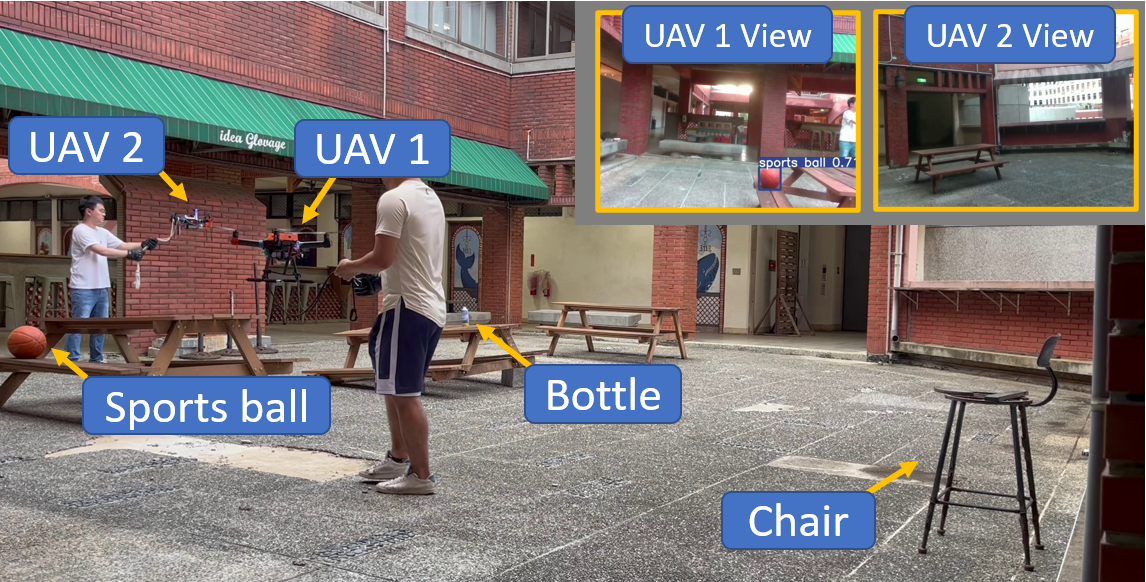
\includegraphics[width=1\textwidth]{exp.png}
        \caption{} \label{GEB exp}
    \end{subfigure}
    \hfill
    \caption{(a) A 13$\times$9 $m.$ public area on the third floor of the General Education Building at the National Central University. (b) An example of UAVs searching for targets (a sports ball, a bottle, and a chair).
    }
    \label{GEB_fig}
\end{figure}

\begin{figure}
  \centering
  \begin{subfigure}[b]{0.5\textwidth}
      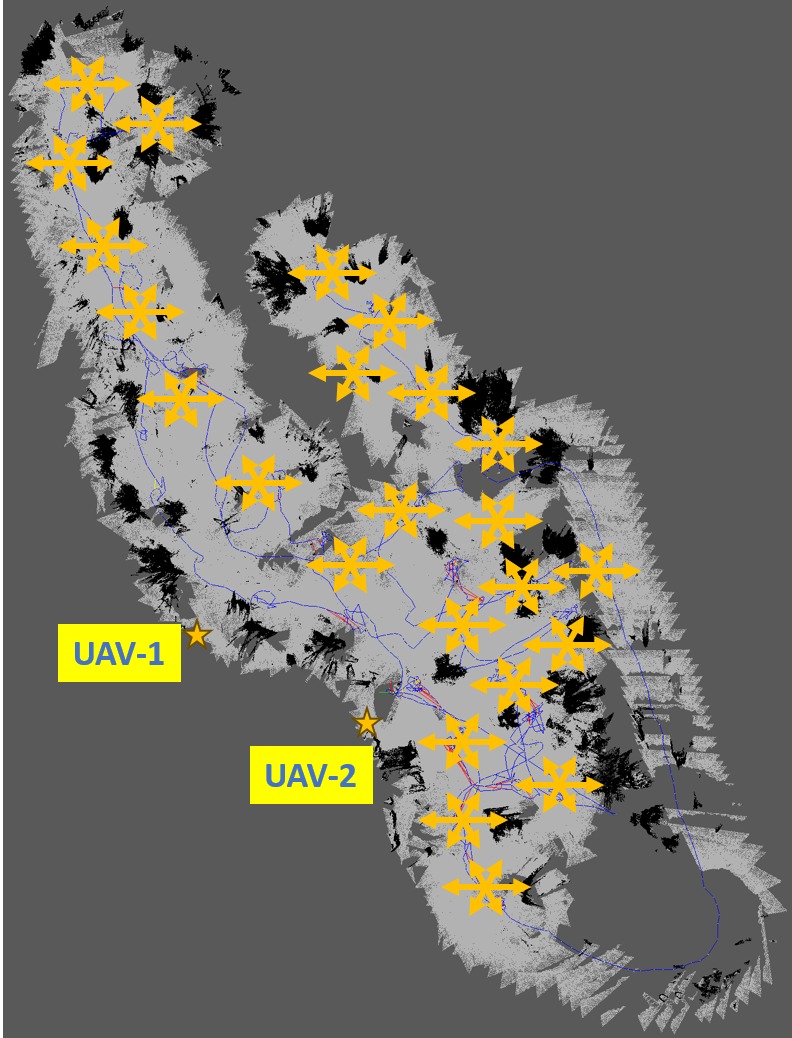
\includegraphics[width=1\textwidth]{map_call.png}
      \caption{} \label{Call map}
  \end{subfigure}
  \begin{subfigure}[b]{0.5\textwidth}
  \centering
      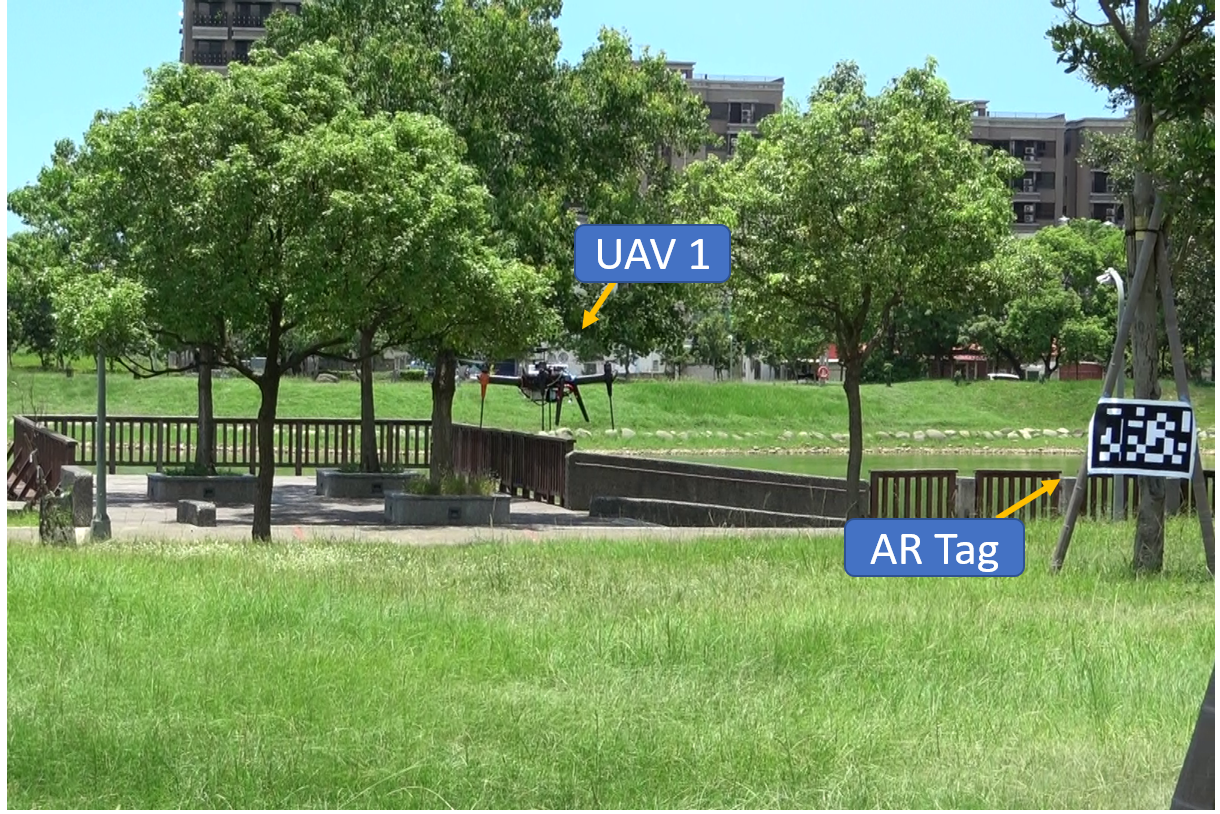
\includegraphics[width=1\textwidth]{Call_uav.png}
      \caption{} \label{Call exp}
  \end{subfigure}
  \hfill
  \caption{(a) A 50$\times$50$\times$5 $m$ lawn at the Hengshan Calligraphy Art Park. (b) An example of a drone searching for AR tags.
  }
  \label{Call_fig}
\end{figure}

\begin{figure}[htbp]
\centerline{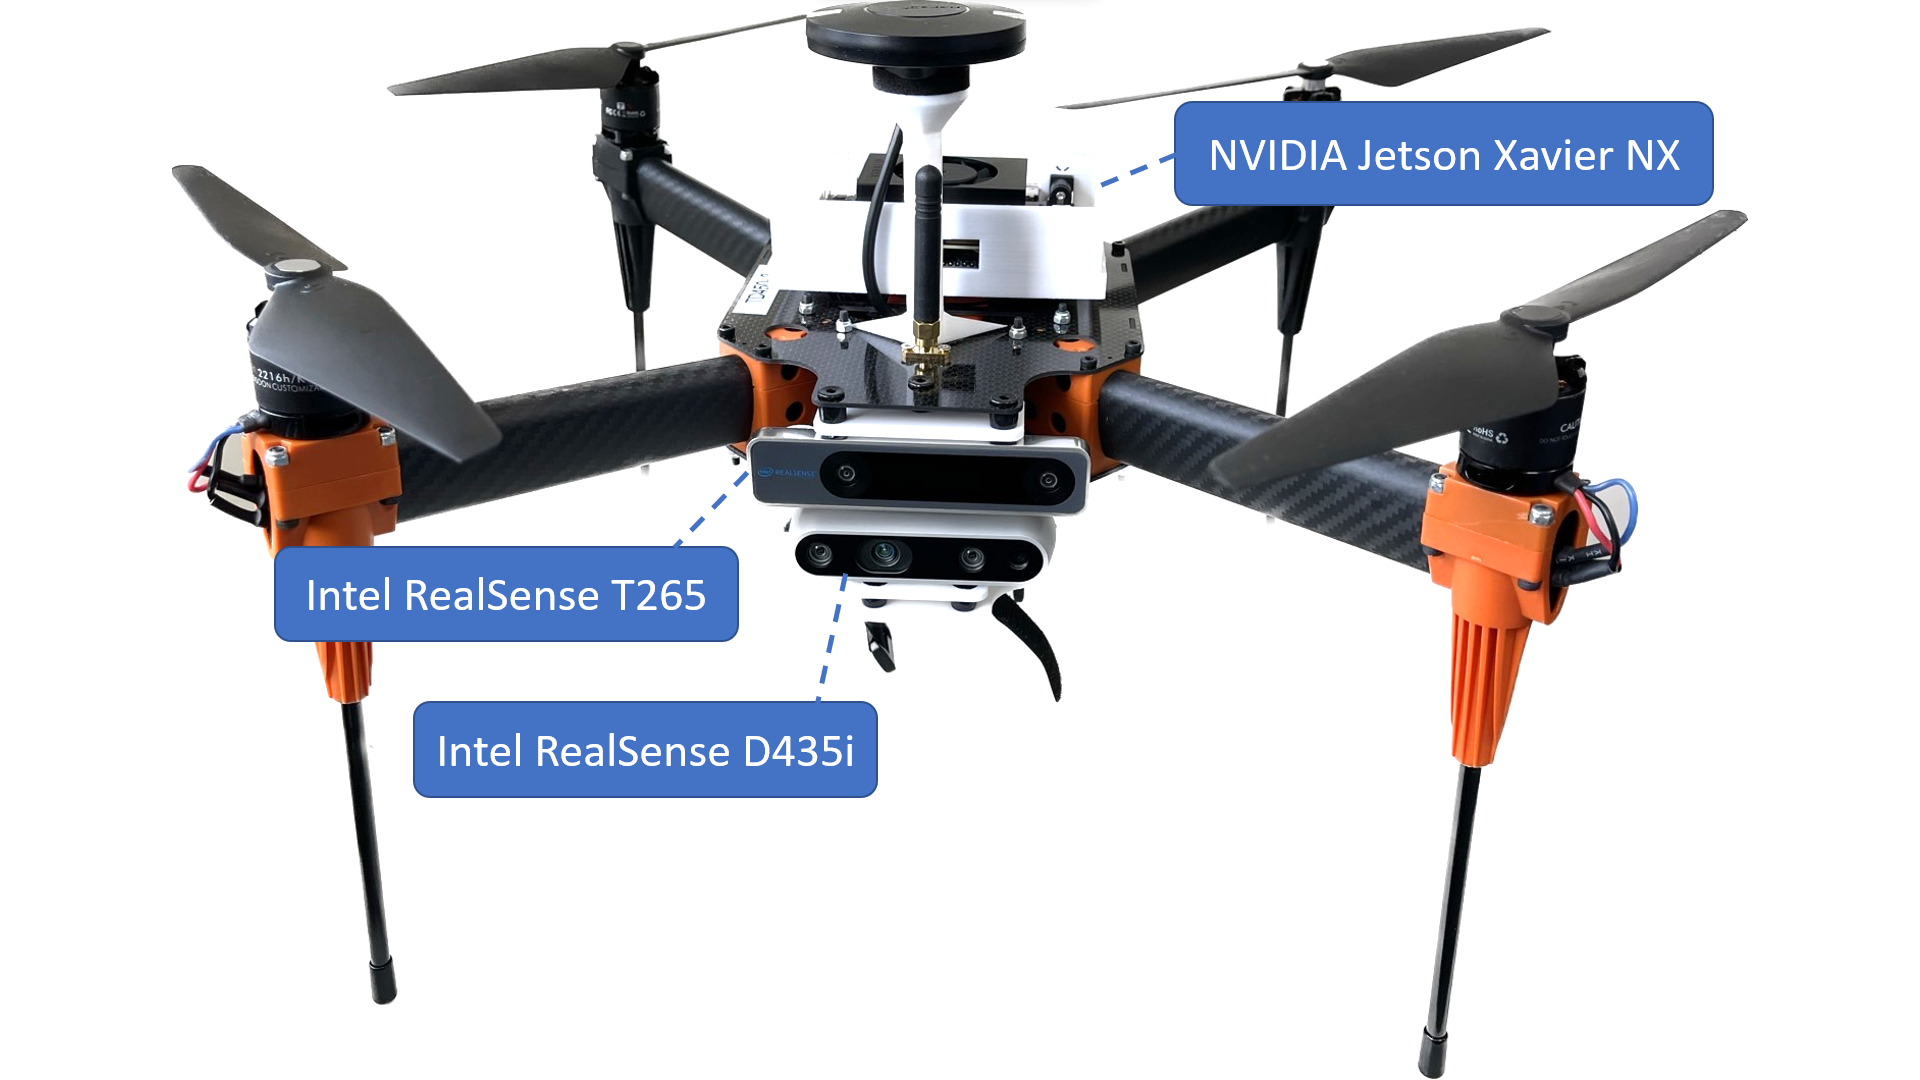
\includegraphics[width=0.6\textwidth]{uav.png}}
\caption{A customized UAV developed by Taiwan Drone 100.}
\label{drone}
\end{figure}

\section{EX$1$: Comparison with Benchmarks on Targets Search}
Table \ref{tab:ANDO} and Table \ref{tab:ETTD} present the simulated performance with a routing budget $l_i=350$, the number of robots $k=3$ and a balancing function weight $\lambda=1$ across various environment sizes.
MRSM is compared to state-of-the-art baselines (e.g., MRSIS\cite{li2024mrsis}, CapAM\cite{paull2022learning}, AM-RL\cite{kool2018attention}, and PD-FAC\cite{sheng2022pd}).

In Table \ref{tab:ANDO}, drones find more objects in a small environment ($a=8$) compared to the larger one ($a=12$).
The decrease in the number of targets in the environment correlates with an increase in the difficulty of the search.
MRSM achieves the highest ENDO in the large environment ($a=12$).
The advantage of MRSM lies in its ability to maximize both the coverage function and the workload balancing function under matroid constraints.
In addition, MRSIS-TSP and MRSM performance is very close in the case of $a=8$. The detailed performance of both MRSM and MRSIS-TSP \cite{li2024mrsis} will be examined in EX2.

Table \ref{tab:ETTD} shows the ETTD of all methods.
All approaches are constrained to search within 10 minutes (600 seconds).
For $a=8$, MRSIS-MST \cite{li2024mrsis} is the most efficient, while for $a=12$, MRSM takes the lead in efficiency.
MRSM, in comparison to AM-RL \cite{kool2018attention}, detects fewer average targets in the $a=8$ scenario.
Despite AM-RL \cite{kool2018attention} finding the highest ENDO, especially within the time constraint of 600 seconds, its search efficiency is compromised due to the largest ETTD value.

To further examine the proposed approaches, algorithms (MRSIS\cite{li2024mrsis}, CapAM\cite{paull2022learning}, and PD-FAC\cite{sheng2022pd}) are evaluated in a real-world environment. Experiments are conducted 5 times for each approach.

In the National Central University scenario, the ETTD and the coverage rate are shown in Table \ref{ETTD table in GEB}.
MRSM achieves an ETTD of 201 seconds and a coverage rate of 67\%, which is the lowest ETTD and the highest coverage rate among other approaches.
Unlike the MST approach (MRSIS-MST \cite{li2024mrsis}), MRSM generates spanning trees that may not be the shortest trajectories, but are the most efficient for target discovery.
The experiments demonstrate that MRSM outperforms benchmark algorithms. In the Hengshan Calligraphy Art Park environment, the ETTD and the coverage rate are shown in Table \ref{ETTD table in Calligraphy}. MRSM outperforms the benchmarks in ETTD, achieving an ETTD of 196 seconds and a coverage rate of 31\%.

The summaries of these experiments are as follows.
The proposed algorithm (MRSM) outperforms state-of-the-art approaches (e.g., MRSIS\cite{li2024mrsis}, AM-RL\cite{kool2018attention}, CapAM\cite{paull2022learning}, and PD-FAC\cite{sheng2022pd}) as claimed in Thm. \ref{def:proposed-bound}.
MRSM achieves the highest coverage rate and discovers targets with the lowest ETTD.
However, it is not guaranteed to find the most targets in the environment.


\begin{table}[h]
  \centering
  \caption{The expected number of detected objects (ENDO) in various environment sizes ($\mathit{\mathbb{E}}$) and number of targets ($\mathit{\mathbb{T}}$) on Gazebo simulator.}
  \label{tab:ANDO}
  \begin{tabular}{ccccccc}
  \toprule
   $\mathit{\mathbb{E}}$ & \multicolumn{3}{c}{8} & \multicolumn{3}{c}{12} \\
  \cmidrule(lr){2-4} \cmidrule(lr){5-7}
   $\mathit{\mathbb{T}}$ & 2 & 4 & 6 & 2 & 4 & 6 \\
  \midrule
  Random & 0.86 & 1.43 & 2.25 & 0.12 & 0.34 & 0.52 \\
  AM-RL & \textbf{1.5} & \textbf{3.15} & \textbf{4.73} & 0.23 & 0.56 & 0.77 \\
  CapAM & 0.89 & 1.69 & 2.48 & 0.34 & 0.81 & 1.18 \\
  PD-FAC & 0.49 & 0.81 & 1.11 & 0.15 & 0.43 & 0.46 \\
  MRSIS-MST & 1.03 & 2.14 & 3.21 & 0.51 & 0.99 & 1.51 \\
  MRSIS-TSP & 1.46 & 2.92 & 4.41 & 1.60 & 3.01 & 4.88 \\
  MRSM & 1.44 & 2.92 & 4.39 & \textbf{1.68} & \textbf{3.19} & \textbf{4.97} \\
  \bottomrule
  \end{tabular}
  \end{table}

  \begin{table}[h]
    \centering
    \caption{The ETTD in various environment sizes ($\mathit{\mathbb{E}}$) and number of targets ($\mathit{\mathbb{T}}$) on Gazebo simulator. The unit is seconds.}
    \label{tab:ETTD}
    \begin{tabular}{ccccccc}
    \toprule
    $\mathit{\mathbb{E}}$ & \multicolumn{3}{c}{$8$} & \multicolumn{3}{c}{$12$} \\
    \cmidrule(lr){2-4} \cmidrule(lr){5-7}
    $\mathit{\mathbb{T}}$ & $2$ & $4$ & $6$ & $2$ & $4$ & $6$ \\
    \midrule
    Random    & $480$ & $438$ & $428$ & $600$ & $600$ & $600$ \\
    AM-RL     & $600$ & $600$ & $600$ & $565$ & $540$ & $518$ \\
    CapAM     & $463$ & $418$ & $377$ & $544$ & $500$ & $463$ \\
    PD-FAC    & $525$ & $450$ & $439$ & $556$ & $497$ & $486$ \\
    MRSIS-MST & $\mathbf{251}$ & $\mathbf{211}$ & $\mathbf{205}$ & $532$ & $478$ & $454$ \\
    MRSIS-TSP & $264$ & $273$ & $259$ & $379$ & $416$ & $386$ \\
    MRSM      & $260$ & $271$ & $258$ & $\mathbf{365}$ & $\mathbf{392}$ & $\mathbf{368}$ \\
    \bottomrule
    \end{tabular}
    \end{table}


\begin{table}[h]
  \centering
  \caption{The ETTD of MRSM and baselines (MRSIS \cite{li2024mrsis}, CapAM \cite{paull2022learning}, and PD-FAC \cite{sheng2022pd}) at the National Central University.}
  \label{ETTD table in GEB}
  \begin{tabular}{cccc}
  \toprule
  Method         & Mean (sec.) & Std. & Coverage Rate \\
  \midrule
  CapAM          & $275$       & $93$ & $42\%$ \\
  PD-FAC         & $314$       & $130$ & $33\%$ \\
  MRSIS-MST      & $206$       & $75$  & $65\%$ \\
  MRSIS-TSP      & $280$       & $58$  & $62\%$ \\
  MRSM           & $\mathbf{201}$ & $93$  & $\mathbf{67\%}$ \\
  \bottomrule
  \end{tabular}
\end{table}

\begin{table}[h]
  \centering
  \caption{The ETTD of MRSM and baselines (MRSIS \cite{li2024mrsis}, CapAM \cite{paull2022learning}, and PD-FAC \cite{sheng2022pd}) at the Hengshan Calligraphy Art Park.}
  \label{ETTD table in Calligraphy}
  \begin{tabular}{cccc}
  \toprule
  Method         & Mean (sec.) & Std. & Coverage Rate \\
  \midrule
  CapAM          & $299$       & $63$ & $22\%$ \\
  PD-FAC         & $268$       & $55$ & $27\%$ \\
  % MRSIS-MST      & $206$       & $75$  & $65\%$ \\
  % MRSIS-TSP      & $280$       & $58$  & $62\%$ \\
  MRSM           & $\mathbf{196}$ & $31$  & $\mathbf{31\%}$ \\
  \bottomrule
  \end{tabular}
\end{table}

%\clearpage
\begin{figure}
   \centering
   \begin{subfigure}[b]{0.45\textwidth}
       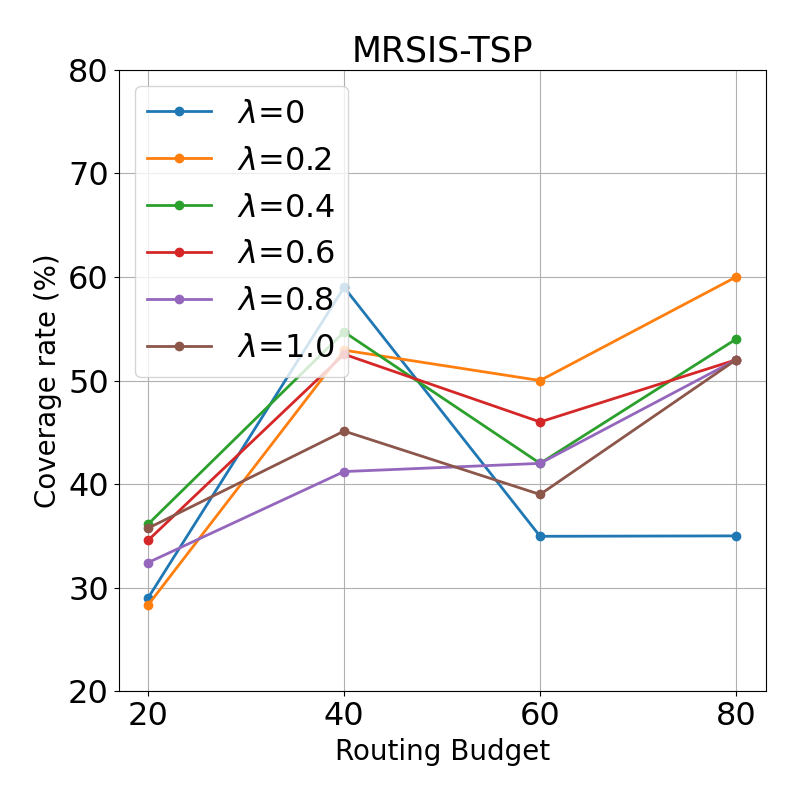
\includegraphics[width=1\textwidth]{MRSIS-TSP-cov.png}
       \caption{MRSIS-TSP\cite{li2024mrsis}}
   \end{subfigure}
   \hfill
   \quad
   \centering
   \begin{subfigure}[b]{0.45\textwidth}
       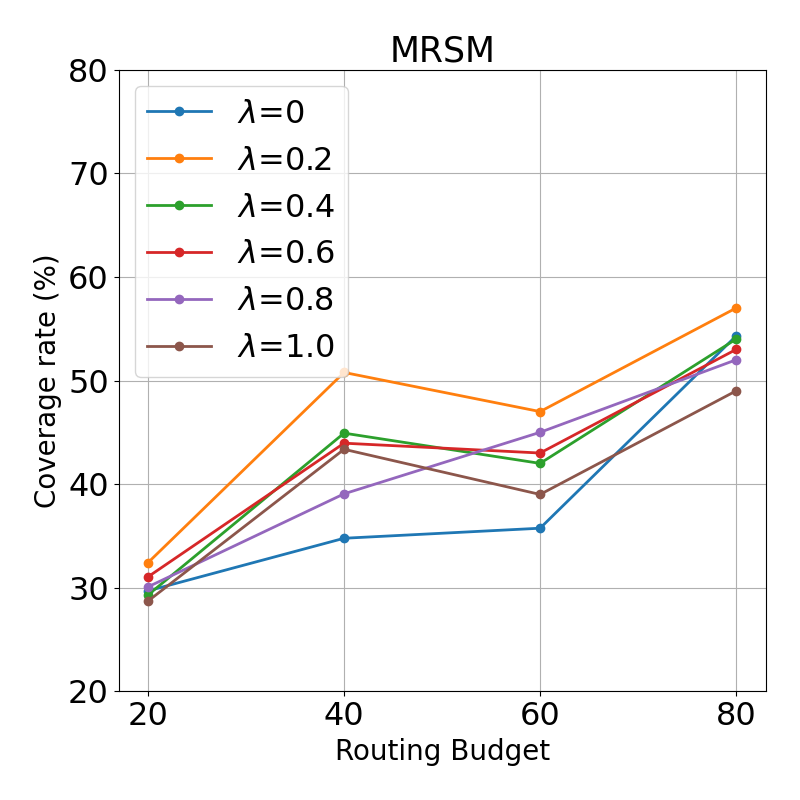
\includegraphics[width=1\textwidth]{MRSM-cov.png}
       \caption{MRSM}
   \end{subfigure}
   \hfill
   \caption{Coverage rate with different robot routing budget $l_i$ and balancing weight $\lambda$.}
   \label{fig:lbd-cov}
\end{figure}

\begin{figure}
   \centering
   \begin{subfigure}[b]{0.45\textwidth}
       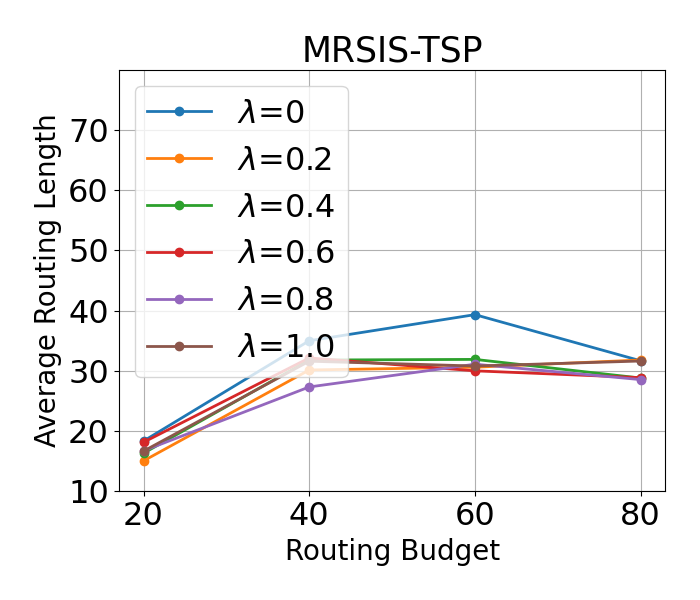
\includegraphics[width=1\textwidth]{MRSIS-TSP.png}
       \caption{MRSIS-TSP\cite{li2024mrsis}}
   \end{subfigure}
   \hfill
   \quad
   \centering
   \begin{subfigure}[b]{0.45\textwidth}
       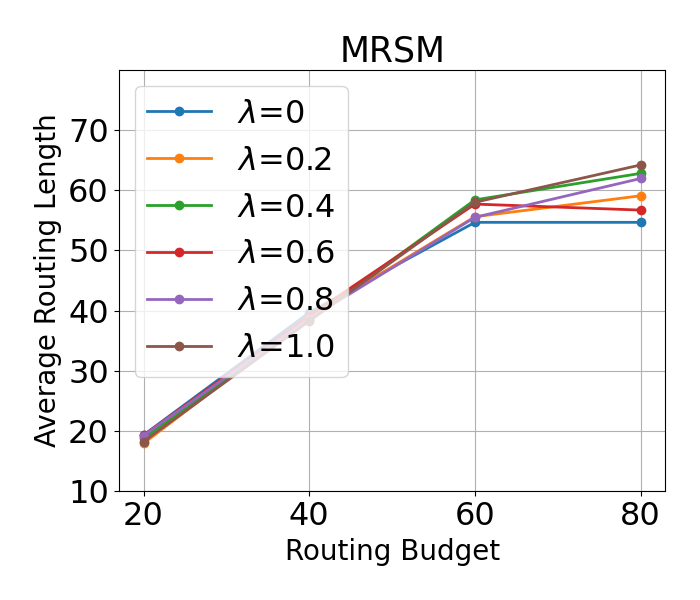
\includegraphics[width=1\textwidth]{MRSM.png}
       \caption{MRSM}
   \end{subfigure}
   \hfill
   \caption{Average routing length (in meters) with various balancing weights $\lambda$ and robot routing budget.}
   \label{fig:routing}
\end{figure}

\begin{table}[h]
  \centering
  \caption{The expected number of detected objects (ENDO) with different parameters (robot routing budget $l_i$, number of targets $b$, and balancing weight $\lambda$) on Gazebo simulator.}
  \label{tab:ANDO-lambda}
  \resizebox{0.6\textwidth}{!}{%
  \begin{tabular}{cccccccccc}
  \toprule
  \multirow{2}{*}{$l_i$} & \multirow{2}{*}{$b$} & \multirow{2}{*}{Method} & \multicolumn{6}{c}{$\lambda$} \\
  \cmidrule(lr){4-9}
   &  &  & 0 & 0.2 & 0.4 & 0.6 & 0.8 & 1 \\
  \midrule
  \multirow{6}{*}{20} & \multirow{2}{*}{2} & MRSIS-TSP & 0.8 & 1.0 & 1.1 & 1.0 & 1.1 & 1.1 \\
   &  & MRSM & \textbf{1.1} & \textbf{1.1} & \textbf{1.2} & \textbf{1.2} & \textbf{1.1} & \textbf{1.1} \\
  \cmidrule(lr){2-9}
   & \multirow{2}{*}{4} & MRSIS-TSP & 1.8 & 2.1 & 2.3 & 2.3 & 2.2 & 2.0 \\
   &  & MRSM & \textbf{2.3} & \textbf{2.2} & \textbf{2.3} & \textbf{2.4} & \textbf{2.2} & \textbf{2.2} \\
  \cmidrule(lr){2-9}
   & \multirow{2}{*}{6} & MRSIS-TSP & 2.6 & 3.2 & 3.4 & 3.4 & 3.2 & 3.1 \\
   &  & MRSM & \textbf{3.4} & \textbf{3.3} & \textbf{3.4} & \textbf{3.6} & \textbf{3.2} & \textbf{3.3} \\
  \midrule
  \multirow{6}{*}{40} & \multirow{2}{*}{2} & MRSIS-TSP & \textbf{1.5} & 1.3 & 1.4 & 1.4 & 1.2 & \textbf{1.5} \\
   &  & MRSM & 1.2 & \textbf{1.4} & \textbf{1.4} & \textbf{1.4} & \textbf{1.3} & 1.3 \\
  \cmidrule(lr){2-9}
   & \multirow{2}{*}{4} & MRSIS-TSP & \textbf{3.2} & 2.8 & 2.8 & \textbf{3.1} & 2.6 & \textbf{3.0} \\
   &  & MRSM & 2.4 & \textbf{2.9} & \textbf{2.8} & 2.9 & \textbf{2.7} & 2.8 \\
  \cmidrule(lr){2-9}
   & \multirow{2}{*}{6} & MRSIS-TSP & \textbf{4.6} & 4.1 & 4.2 & \textbf{4.5} & 3.8 & \textbf{4.5} \\
   &  & MRSM & 3.5 & \textbf{4.5} & \textbf{4.3} & 4.3 & \textbf{4.1} & 4.1 \\
  \midrule
  \multirow{6}{*}{60} & \multirow{2}{*}{2} & MRSIS-TSP & \textbf{1.3} & \textbf{1.0} & \textbf{1.0} & \textbf{1.0} & \textbf{1.0} & \textbf{1.0} \\
   &  & MRSM & 1.3 & 0.9 & 0.9 & 0.9 & 0.9 & 0.9 \\
  \cmidrule(lr){2-9}
   & \multirow{2}{*}{4} & MRSIS-TSP & 2.6 & \textbf{2.2} & \textbf{2.0} & \textbf{2.2} & \textbf{2.2} & \textbf{2.1} \\
   &  & MRSM & \textbf{2.7} & 2.1 & 1.9 & 2.0 & 2.0 & 1.8 \\
  \cmidrule(lr){2-9}
   & \multirow{2}{*}{6} & MRSIS-TSP & 3.7 & \textbf{3.3} & \textbf{3.0} & \textbf{3.2} & \textbf{3.3} & \textbf{3.2} \\
   &  & MRSM & \textbf{4.0} & 3.1 & 2.9 & 2.9 & 3 & 2.8 \\
  \midrule
  \multirow{6}{*}{80} & \multirow{2}{*}{2} & MRSIS-TSP & 1.3 & \textbf{1.5} & \textbf{1.5} & 1.4 & \textbf{1.4} & \textbf{1.4} \\
   &  & MRSM & \textbf{1.5} & 1.4 & 1.5 & \textbf{1.5} & 1.4 & 1.4 \\
  \cmidrule(lr){2-9}
   & \multirow{2}{*}{4} & MRSIS-TSP & 2.7 & \textbf{3.2} & \textbf{3.0} & 2.8 & 2.9 & \textbf{3.1} \\
   &  & MRSM & \textbf{3.1} & 3.1 & 3.0 & \textbf{3.1} & \textbf{3.0} & 2.9 \\
  \cmidrule(lr){2-9}
   & \multirow{2}{*}{6} & MRSIS-TSP & 4 & \textbf{4.6} & \textbf{4.4} & 4.1 & 4.3 & \textbf{4.4} \\
   &  & MRSM & \textbf{4.7} & 4.4 & 4.4 & \textbf{4.5} & \textbf{4.4} & 4.3 \\
  \bottomrule
  \end{tabular} }
  \end{table}


  \begin{table}[h]
  \centering
  \caption{The ETTD with different parameters (robot routing budget $l_i$, number of targets $b$, and balancing weight $\lambda$) on Gazebo simulator. The unit is in seconds.}
  \label{tab:ETTD-lambda}
  \resizebox{0.6\textwidth}{!}{%
  \begin{tabular}{ccccccccc}
  \hline
  \multirow{2}{*}{$l_i$} & \multirow{2}{*}{$b$} & \multirow{2}{*}{Method} & \multicolumn{6}{c}{$\lambda$} \\ \cline{4-9}
   &  &  & 0 & 0.2 & 0.4 & 0.6 & 0.8 & 1 \\ \hline
  \multirow{6}{*}{20} & \multirow{2}{*}{2} & MRSIS-TSP & 384 & 342 & 335 & 347 & 328 & 342 \\
   &  & MRSM & \textbf{326} & \textbf{315} & \textbf{303} & \textbf{282} & \textbf{323} & \textbf{328} \\ \cline{2-9}
   & \multirow{2}{*}{4} & MRSIS-TSP & 382 & 340 & \textbf{313} & 325 & 337 & 355 \\
   &  & MRSM & \textbf{308} & \textbf{313} & 315 & \textbf{292} & \textbf{317} & \textbf{328} \\ \cline{2-9}
   & \multirow{2}{*}{6} & MRSIS-TSP & 378 & 334 & \textbf{313} & 316 & 330 & 348 \\
   &  & MRSM & \textbf{309} & \textbf{313} & 314 & \textbf{292} & \textbf{327} & 320 \\ \hline
  \multirow{6}{*}{40} & \multirow{2}{*}{2} & MRSIS-TSP & \textbf{272} & 302 & 282 & 271 & 316 & \textbf{258} \\
   &  & MRSM & 309 & \textbf{261} & \textbf{278} & \textbf{261} & \textbf{293} & 300 \\ \cline{2-9}
   & \multirow{2}{*}{4} & MRSIS-TSP & \textbf{251} & 275 & 289 & \textbf{249} & 292 & \textbf{261} \\
   &  & MRSM & 329 & \textbf{264} & \textbf{286} & 252 & \textbf{279} & 273 \\ \cline{2-9}
   & \multirow{2}{*}{6} & MRSIS-TSP & \textbf{260} & 278 & 277 & 249 & 292 & \textbf{247} \\
   &  & MRSM & 320 & \textbf{246} & \textbf{255} & \textbf{244} & \textbf{277} & 269 \\ \hline
  \multirow{6}{*}{60} & \multirow{2}{*}{2} & MRSIS-TSP & \textbf{307} & \textbf{266} & \textbf{270} & \textbf{283} & \textbf{266} & \textbf{297} \\
   &  & MRSM & 308 & 317 & 318 & 307 & 324 & 328 \\ \cline{2-9}
   & \multirow{2}{*}{4} & MRSIS-TSP & \textbf{310} & \textbf{195} & \textbf{203} & \textbf{223} & \textbf{205} & \textbf{226} \\
   &  & MRSM & 312 & 229 & 271 & 243 & 238 & 249 \\ \cline{2-9}
   & \multirow{2}{*}{6} & MRSIS-TSP & 321 & \textbf{159} & \textbf{158} & \textbf{190} & \textbf{148} & \textbf{179} \\
   &  & MRSM & \textbf{301} & 205 & 231 & 194 & 209 & 204 \\ \hline
  \multirow{6}{*}{80} & \multirow{2}{*}{2} & MRSIS-TSP & 313 & \textbf{277} & \textbf{273} & 286 & \textbf{275} & \textbf{263} \\
   &  & MRSM & \textbf{269} & 288 & 274 & \textbf{273} & 286 & 280 \\ \cline{2-9}
   & \multirow{2}{*}{4} & MRSIS-TSP & 293 & \textbf{256} & \textbf{275} & 288 & \textbf{266} & \textbf{242} \\
   &  & MRSM & \textbf{286} & 257 & 280 & \textbf{267} & 279 & 290 \\ \cline{2-9}
   & \multirow{2}{*}{6} & MRSIS-TSP & 291 & \textbf{260} & 274 & 286 & \textbf{256} & \textbf{249} \\
   &  & MRSM & \textbf{271} & 270 & \textbf{271} & \textbf{262} & 269 & 278 \\ \hline
  \end{tabular} }
  \end{table}


  \begin{table}[]
    \centering
    \caption{The ENDO of MRSM with different parameters (environment sizes $\mathbb{E}$, number of targets $b$, and balancing weights $\lambda$) on Gazebo simulator.}
    \label{tab:ENDO-Env-lambda}
    \begin{tabular}{ccllllll}
    \hline
    \multirow{2}{*}{$\mathbb{E}$} & \multirow{2}{*}{$b$} & \multicolumn{6}{c}{$\lambda$}                                                                 \\ \cline{3-8}
     &
       &
      \multicolumn{1}{c}{0} &
      \multicolumn{1}{c}{0.2} &
      \multicolumn{1}{c}{0.4} &
      \multicolumn{1}{c}{0.6} &
      \multicolumn{1}{c}{0.8} &
      \multicolumn{1}{c}{1} \\ \hline
    \multirow{3}{*}{8} &
      2 &
      1.62 &
      \textbf{1.96} &
      \textbf{1.96} &
      \textbf{1.96} &
      \textbf{1.96} &
      1.91 \\
                         & 4                    & 3.18          & 3.87          & 3.88          & 3.90          & 3.86          & \textbf{3.92} \\
                         & 6                    & 4.91          & 5.90          & \textbf{5.91} & 5.89          & 5.85          & 5.87          \\ \hline
    \multirow{3}{*}{10}  & 2                    & 1.55          & \textbf{1.68} & 1.53          & 1.60          & 1.54          & 1.57          \\
                         & 4                    & 2.80          & 3.19          & 3.16          & 3.23          & 3.06          & \textbf{3.33} \\
                         & 6                    & 4.25          & 4.88          & 4.72          & 4.98          & 4.58          & \textbf{5.04} \\ \hline
    \multirow{3}{*}{12}  & 2                    & 1.02          & 0.92          & 1.09          & 0.97          & 1.08          & \textbf{0.97} \\
                         & 4                    & 1.83          & 1.99          & 2.07          & 1.89          & \textbf{2.25} & 1.74          \\
                         & 6                    & 2.88          & 3.03          & \textbf{3.13} & 2.84          & 2.90          & 2.75          \\ \hline
    \multirow{3}{*}{14}  & 2                    & \textbf{0.68} & 0.62          & 0.58          & 0.61          & 0.64          & 0.54          \\
                         & 4                    & 1.18          & 1.04          & 1.00          & \textbf{1.19} & 1.01          & 1.02          \\
                         & 6                    & 1.65          & 1.77          & 1.62          & \textbf{1.69} & 1.68          & 1.46          \\ \hline
    \end{tabular}
    \end{table}



    \begin{table}[]
    \centering
    \caption{The ETTD of MRSM with different parameters (environment sizes $\mathbb{E}$, number of targets $b$, and balancing weights $\lambda$) on Gazebo simulator. The unit is in seconds.}
    \label{tab:ETTD-Env-lambda}
    \begin{tabular}{ccllllll}
    \hline
    \multirow{2}{*}{$\mathbb{E}$} &
      \multirow{2}{*}{$b$} &
      \multicolumn{6}{c}{$\lambda$} \\ \cline{3-8}
     &
       &
      \multicolumn{1}{c}{0} &
      \multicolumn{1}{c}{0.2} &
      \multicolumn{1}{c}{0.4} &
      \multicolumn{1}{c}{0.6} &
      \multicolumn{1}{c}{0.8} &
      \multicolumn{1}{c}{1} \\ \hline
    \multirow{3}{*}{8}  & 2 & 200          & 125          & 127          & 128          & \textbf{122} & 141          \\
                        & 4 & 207          & 130          & 135          & \textbf{125} & 133          & 131          \\
                        & 6 & 196          & \textbf{121} & 129          & 128          & 129          & 131          \\ \hline
    \multirow{3}{*}{10} & 2 & 217          & \textbf{179} & 212          & 190          & 208          & 209          \\
                        & 4 & 257          & 202          & 198          & 184          & 211          & \textbf{183} \\
                        & 6 & 251          & 195          & 199          & \textbf{173} & 212          & 180          \\ \hline
    \multirow{3}{*}{12} & 2 & 337          & 360          & \textbf{313} & 345          & 320          & 344          \\
                        & 4 & 366          & 340          & 332          & 353          & \textbf{310} & 370          \\
                        & 6 & 354          & 337          & \textbf{329} & 351          & 352          & 357          \\ \hline
    \multirow{3}{*}{14} & 2 & \textbf{420} & 435          & 447          & 440          & 431          & 458          \\
                        & 4 & \textbf{445} & 461          & 468          & \textbf{445} & 468          & 465          \\
                        & 6 & 455          & \textbf{443} & 457          & 451          & 453          & 471          \\ \hline
    \end{tabular}
    \end{table}


\section{EX$2$: Parametric Analysis}
To verify the parametric analysis of MRSIS-TSP\cite{li2024mrsis} and MRSM, the parameters (the coverage rate, the average routing length, the ENDO, and the ETTD) are compared in various balancing weights ($\lambda$) and robot routing budgets ($l_i$).

The coverage rate of MRSIS-TSP\cite{li2024mrsis} and MRSM under different balancing weights ($\lambda$) and robot routing budgets ($l_i$) is as follows.
Fig. \ref{fig:lbd-cov}(a) illustrates the coverage rate of MRSIS-TSP\cite{li2024mrsis}.
When $\lambda=0$, a substantial variance exists among the routing budgets.
No balancing function outperforms at $l_i=40$ while performing less effectively in other cases.
Besides, a smaller balancing weight demonstrates effective performance.
At $l_i=20$, $l_i=60$, and $l_i=80$, a small magnitude of the balancing weight performs optimally.
At $l_i=40$, no balancing function ranks the highest. However, when the balancing function is considered, $\lambda=0.4$ achieves the highest coverage rate.
Fig. \ref{fig:lbd-cov}(b) illustrates the coverage rate of MRSM.
The weight $\lambda=0.2$ yields the highest coverage rate across all routing budget cases.
Besides, the coverage rate of MRSM is more consistent than that of MRSIS-TSP\cite{li2024mrsis}.

Fig. \ref{fig:routing} illustrates the average routing length on 3 robots with various balancing weights ($\lambda$) and robot routing budgets ($l_i$).
As the routing budget increases, robots cover larger traveling distances.
The routing length converges due to the limitation of environment size.
In MRSIS-TSP\cite{li2024mrsis} scenario (Fig. \ref{fig:routing}(a)), robots travel between 10 and 40 meters.
In MRSM scenario (Fig. \ref{fig:routing}(b)), the traveled distance is between 20 and 65 meters.
The reason for the smaller routing distance in MRSIS-TSP\cite{li2024mrsis} compared to MRSM is that MRSIS-TSP\cite{li2024mrsis} utilizes a TSP approximator to minimize travel distances.
Therefore, the average routing length of MRSM is more than that of MRSIS-TSP\cite{li2024mrsis}.

Table \ref{tab:ANDO-lambda} and Table \ref{tab:ETTD-lambda} show the ENDO and the ETTD, respectively.
The best performance is highlighted in bold.
The results indicate that no single method consistently outperforms in all cases.
On average, MRSM outperforms in 38 out of 72 cases, while MRSIS-TSP\cite{li2024mrsis} achieves superiority in 34 out of 72 cases.
Additionally, MRSM excels in small routing budgets ($l_i\leq40$), while MRSIS-TSP\cite{li2024mrsis} performs well in the larger ones.
Since MRSIS-TSP\cite{li2024mrsis} inherits the routing minimization feature, it has an advantage in larger routing budgets by facilitating efficient travel.
Moreover, in some cases, the performance is superior when the balancing function is not involved.
Since the proposed objective function is defined as $F(S)=f(S)+\lambda \mathcal{B}(S)$, when $\lambda=0$, the objective function is simply a coverage function.
Optimizing the coverage function with routing and clustering constraints may yield good performance in certain cases.

To elucidate the use of parameters, Table \ref{tab:ENDO-Env-lambda} and Table \ref{tab:ETTD-Env-lambda} show the performance (ENDO and ETTD) of MRSM in various environment sizes and number of targets. Small environments allow for faster target detection compared to large ones. While no single lambda value is optimal for all environment sizes, empirical results indicate that small environments benefit from larger lambda values, whereas large environments can perform well with smaller lambda values. As the environment size increases, the results suggest that a large area can be covered even with an imbalance in workload distribution.


The EX2 results demonstrate that a small balancing weight magnitude leads to optimal performance for both MRSM and MRSIS-TSP \cite{li2024mrsis}. Across most cases, MRSM outperforms MRSIS-TSP \cite{li2024mrsis} due to the theoretical guarantee of submodularity under matroid constraints. In contrast, smaller environments require a more balanced workload assignment to optimize performance.



\section{EX$3$: Scalability Analysis}
Table \ref{tab:large-scale-SG} shows the performance of MRSM, CapAM \cite{paull2022learning}, and PD-FAC \cite{sheng2022pd} with various number of robots (UAVs) and subgoals. The coverage rate increases with the number of subgoals. The results show that MRSM outperforms the benchmarks in ENDO, ETTD, and coverage rate.

In summary, due to the theoretical guarantee of submodularity, when the number of subgoals and robots increases, the coverage rate does not deteriorate. In addition, MRSM outperforms state-of-the-art methods for multi-robot search scenarios.
\begin{table}[]
  \centering
  \caption{Large-scale experiment results of the ENDO, the ETTD, and the coverage rate with different numbers of subgoals and UAVs on Gazebo simulator.}
  \label{tab:large-scale-SG}
  \resizebox{0.6\textwidth}{!}{%
  \begin{tabular}{cccccc}
  \hline
  No. Subgoals & No. UAVs & Method & ENDO & ETTD & Coverage rate \\ \hline
  \multirow{6}{*}{700} & \multirow{3}{*}{5}  & CapAM  & 5.49 & 551 & 66\% \\
                       &                     & PD-FAC & 3.87 & 413 & 47\% \\
                       &                     & MRSM   & \textbf{6.24} & \textbf{290} & \textbf{73\%} \\ \cline{2-6}
                       & \multirow{3}{*}{10} & CapAM  & 6.13 & 514 & 73\% \\
                       &                     & PD-FAC & 4.52 & 381 & 53\% \\
                       &                     & MRSM   & \textbf{6.23} & \textbf{238} & \textbf{75\%} \\ \hline
  \multirow{6}{*}{800} & \multirow{3}{*}{5}  & CapAM  & 4.68 & 514 & 58\% \\
                       &                     & PD-FAC & 4.75 & 383 & 56\% \\
                       &                     & MRSM   & \textbf{6.42} & \textbf{280} & \textbf{75\%} \\ \cline{2-6}
                       & \multirow{3}{*}{10} & CapAM  & 6.17 & 534 & 73\% \\
                       &                     & PD-FAC & 4.35 & 376 & 59\% \\
                       &                     & MRSM   & \textbf{6.43} & \textbf{257} & \textbf{77\%} \\ \hline
  \multirow{6}{*}{900} & \multirow{3}{*}{5}  & CapAM  & 4.92 & 496 & 58\% \\
                       &                     & PD-FAC & 4.08 & 416 & 51\% \\
                       &                     & MRSM   & \textbf{6.87} & \textbf{256} & \textbf{77\%} \\ \cline{2-6}
                       & \multirow{3}{*}{10} & CapAM  & 5.98 & 506 & 72\% \\
                       &                     & PD-FAC & 4.4 & 354 & 53\% \\
                       &                     & MRSM   & \textbf{6.93} & \textbf{243} & \textbf{82\%} \\ \hline
  \end{tabular} }
  \end{table}
